\section{Background.}
\label{sec:background}

\subsection{Pipeline of ERD Processing.}

The process of recognizing and disambiguating the entities in a text usually follows a three-step pipeline, in which each of the steps is essential to let the next step work correctly. In this Subsection we present each of these steps, which we will describe later in subsequent Subsections.

We expose the basic structure of the pipeline in \autoref{fig:pipeline}. First, we need to pre-process the raw text to standardize the input for the next steps. As we pointed in the introduction of this paper, the nature of a natural language text is very diverse, and it can be difficult, or almost impossible, to build a system that is able to face every challenge that a text can present. This step is important too to optimize the computational cost of the later operations, as we can filter which parts of the input text are relevant for our purposes.

\begin{figure}[!ht]
\centering
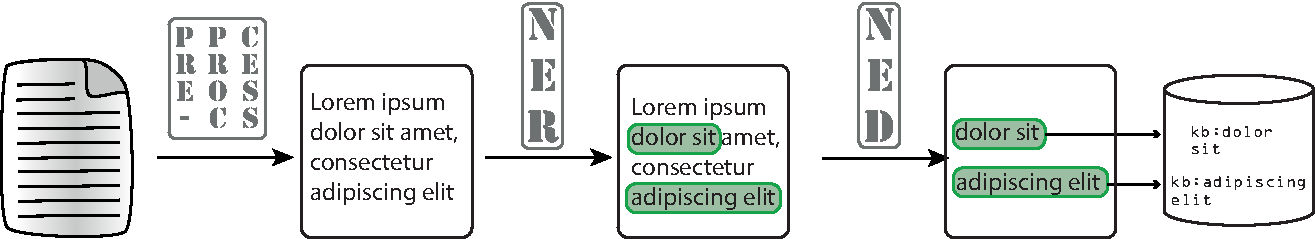
\includegraphics[width=.9\textwidth]{pipeline}

\caption{Overview of the NERD pipeline {\color{red}(provisional)}.}
\label{fig:pipeline}
\end{figure}%

\begin{comment}
Once we have pre-processed the original input text, we use the result as input for the ER component. This component has two main goals that carries out sequentially: first, it detects which words or expressions are able to represent one or more entities in that text. This expressions are usually called \emph{mentions}. This is not a trivial operation: some words may or may not be a mention depending on the surrounding text, as we will see later; and it can be some mentions that our system cannot be able to recognise as such. After this step, a generic NER module should be able to gather a list of candidate entities from the knowledge base for each one of the detected mentions.
\end{comment}

Once we have pre-processed the original input text, we use the result as input for the ER component. This component should find all the entities that are present in the text. These \emph{mentions} can be explicit or implicit, being the first case the most frequent in the state of art, although there are some works that are specialized in the latter one, like \cite{perera2016}. A general approach is the partial or exact match of a sequence of words with an entry in the surface form dictionary. 

Every entity can be called with one or more names; we call each one of these names a \emph{surface form} of a certain entity. As well as one entity can have many surface forms, the same surface form can be used for naming many entities (remember our initial example, where \textit{Born to Run} can be both the album and the song). A surface form dictionary gather all the known surface forms for each entity that is described in the used knowledge base, and relates the former with the latter. They are also known as mention dictionaries.

The desired output of the ER phase is a list of words or phrases that may represent an entity in the text, although we do not know which entities are referred to in it.

\begin{defi}[{\bf Entity}]
An entity is an element from reality that can be called using a name, proper or not, and has a set of properties that describes and characterizes it. People, places, concepts and anything are examples of usual entities. The set of characteristics that describes an entity depends on the needs of each NERD system.
\end{defi}

\begin{defi}[{\bf Mention}]
A mention is a word or phrase in a text that may represent an entity in a natural language text. The mention text should match partially or exactly one of the surface forms that can be recognized by our NER system, or be a pronoun that replaces an entity already mentioned in the text. 
\end{defi}

\begin{defi}[{\bf Surface form}]
A surface form is a possible name (word or phrase) that can be used to refer to an entity in a text. Usually there is many alternative names for the same entity, whilst one of them stands as the \emph{canonical name}, e.g. the most probable one or the one used as title in the corresponding article in Wikipedia. First names and surnames, alias or alternative forms are frequent examples of surface forms.
\end{defi}

The last step in our pipeline is the disambiguation. This occurs in two phases: first, we need to gather the entities that can be represented by each of the mentions provided by the ER component. Second, we need to choose the best candidate in the set of candidate entities for each one of the mentions. 

In the first step, we use the surface form dictionary. This way, we are able to get a set of candidate entities for each identified mention. In case of finding two or more candidate entities for at least one mention in the text, it is needed a disambiguation phase to determine which of the candidate entities fits best as the represented entity by the ambiguous mention. If every mention has exactly one possible entity to correspond with, the annotation is immediate.

If there are many entities that can be assigned to a mention, the disambiguation component must decide which may be the most appropriate. The proposed solutions to this problem are varied, and are the main focus of our paper. In subsequent sections, we delve in the most common approaches and techniques that are used to identify the candidate entity that best fit as the correct annotation for each mention.

The output of a standard ERD pipeline is a list of mentions and their linked entities, frequently embedding the results in the original text by replacing the mentions with hyperlinks. Some additional information can be provided to improve the significance of this result, like lists of candidates, the value of the factor used to decide the best candidate, etcetera.

\medskip

An optional task that is performed in some proposals consists on a final clustering of all mentions that could not be linked with any resource. This let us gather all the similar mentions of this kind across the whole input text, or in a document corpora that is being processed. A general solution is tagging these entities with an empty or null resource. Later we will delve into the implications of this kind of resource.

\bigskip

\noindent\textbf{ERD Challenges}~

The ERD process has many characteristic difficulties that are widely described in all the related bibliography. The most important three ones are listed in \cite{rao2013}, to which we add a fourth: false mentions. Below we briefly describe each one of the problems that we have to face when trying to recognize and disambiguate the entities in a text:

\paragraph{False mentions} As we pointed before, a word or phrase can be or not a mention depending on multiple factors: its grammatical category, its surrounding context, the desired domain for the ERD system (which can bring some semantic idiosyncrasy to the recognition problem), and so on. An accurate ER system must take into account these and other factors to do its task, so it can provide accurate and relevant results to the ED system.

\paragraph{Name variation} One of the main problems in the ER step of the process is related to synonymy. Although any entity can have a conveyed canonical name (which is important to identify it in a computational way), it can also have one or more alternative forms in which it can appear in a text. It can happen in two manners: the explicit way, in which there exists another name for the entity (e.g. Bruce Springsteen and \emph{The Boss}), and the implicit way, where the entity is implicit in a word or phrase that is not just an alternative name, like when we use a pronoun or a more generic denomination to identify an specific object of a class (e.g. ``the Springsteen's album of 1975'' instead of \textit{Born to Run}).

First case is easier to tackle: the number of possible denominations for an entity is limited, so having a complete and up to date knowledge base should be enough to recognize all of the possible manifestations of each entity. This would let us to know about every surface form that should be recognized by our system. The second one requires a more complex processing by inferring the semantics behind the text: to correctly detect the ``Springsteen's album of 1975'' as a mention to \textit{Born to Run}, a system should know about previous mentions in the text to an entity that fits that description. This action would require that the system could be able to recognize, understand and check the semantic relations between entities.

\paragraph{Mention ambiguity} This is the complementary problem of the previous one: the same word or phrase can be used to call two or more entities, which is the fact that motivates the need of disambiguation. Following our working example, we can see this phenomenon with the mention \textit{Born to Run}, as it may refer to both the album, the song or even the recent autobiographical book by Springsteen. However, not having any ambiguity in a text is not always good news, as it can be an indicative of a lack of information in our knowledge base. 

\paragraph{Entity absence} This problem sums up the two previous problems, and can motivate both of them. If we do not have information about a certain entity, we can not determine which surface forms can represent it in a text, therefore we will not be able to recognise them in a text and it will not be considered during the disambiguation phase.

The main reasons for a possible lack of information are three: having selected a bad source for building the knowledge base, having used wrong procedures to extract the information from that source, or working with an obsolete (thus, not up to date with the new information that is generated every day) knowledge base.



\subsection{Fundamentals of Natural Language Processing.}

The pre-processing of an input text makes use of some common NLP techniques, which are discussed below. 

\paragraph{Text Tokenization}
The first step is to modify the structure of the input text to ease the automatic process of it. Generally, text tokenization (or text segmentation) consists on divide the text in more manageable units, like words or sentences. We will focus in the concept of token as words, as it is more useful to ERD than just sentences.

At a first glance, this can seem an easy task, but it is not. Words are not only separated by blank spaces; instead, we can use a plethora of punctuation symbols like dots, commas and more. There are some idiosyncratic aspects that must be faced depending on the language used for writing a text; e.g. in English we have the saxon genitive, in Arabic there are not blank spaces...

Each of these peculiarities must be tackled by defining specific rules to improve the performance over a system that applies only a set of generic rules. The output of this process provides a more manageable set of elements to work with, as it let us to detect possible mentions between these tokens, or to build different combinations of those to be able to recognize multi-word mentions.

\paragraph{Stopword Removal}
One thing that we must take into account in NERD process is the computational cost of it. One good idea could be to reduce the total number of elements that we use as input for the NERD pipeline. To accomplish this, we can exploit the fact that, in every text, there are some words that have no own sense, and they are used instead to make consistent that text. Additionally, there is a large portion of words that cannot be (or it is unlikely enough to ignore them) a mention, so they can be removed from the input to the entity recognition module.

This way, we can prune prepositions, determinants, conjunctions, and so on. We must be careful, though: some stop words can be part of an entities name, e.g. the particle \emph{to} in the album title \textit{Born to Run}, so deleting them might not be that safe and can lead to poor entity recognition performance. For this reason, this operation is more frequent in other areas, such as information retrieval, and is not implemented as part of the NERD pipeline.

\paragraph{POS Tagging}
The Part-of-Speech tagging is one of the most useful operations in the pre-processing step. What it does is to process an input text, detecting and labeling words or a set of words with their grammatical category. It can be done in two ways: by tagging each word as noun, verb, adjective, etcetera; or by identifying the function of each phrasal element, like noun or pronoun phrase, verbal phrase, and so on.

The difficulty of this operation are those words or phrases whose category may be ambiguous, e.g. some words can be identified as verbs or nouns depending on the surrounding context. A correct POS Tagging is very important for NERD, as long as many systems can ignore all words that are not a noun or pronoun to reduce the required computation load, memory usage and general complexity. If a system puts a wrong label, an important mention to an entity could remain hidden to our NERD system.

\paragraph{Stemming}
The stemming is not a common operation in ERD, being more useful in terms of information retrieval, but it follows the mentioned principle of standardize the input to ease its processing. This task consists on replacing each word that is derived from a root form (for instance, conjugated verbs or plural forms of nouns) with that root form. This way we reduce the complexity of the text by limiting the elements which a text can be constructed with.

\subsection{Named Entities.}

Traditionally, the works in ERD has been focused in what has been called \emph{named entities}. Traditionally, this fact motivated the use of the name NERD instead of ERD, which stands for Named Entity Recognition and Disambiguation. Named entities are all those elements from reality that can be identified in an univocal manner with a proper name. The elements that fulfil this definition can generally be distributed en three categories: Person, Location and Organizations. Some authors extends this classification with a fourth class, Miscellaneous, or even a fifth, Events (as proposed in YAGO \cite{yago2007}).

Seminal works in this area considered only entities of this kind, but later, and thanks to the influence of Wikipedia (which has an encyclopedic nature, thus not restricted to only named entities), more and more proposals extended his functionality to what has been called \emph{conceptual entities}, or just entities. This denomination refers to every element in reality that can be named, like concepts, emotions, historical periods... This evolution brings a higher complexity of the process, but greatly increases the functionality of the classic NERD systems. At this point, we consider that the ERD denomination may be more accurate, instead of keep using the NERD name, as it does not limit to the named entities any more.

The chosen approach often depends on the objective of the ERD system: for instance, the first approach is better for a system that is used for automatically enrich news articles, where the relevant entities are people that take part in events that occur in a specific place. On the other hand, a system oriented to verify the correctness of the links between a set of Wikipedia articles could use a broader concept of entity.

\begin{defi}[{\bf Named Entity}]
Named entities are those that are called with proper names, that is, they are unique and recognizable only as themselves. In general, named entities refers to people, organizations and places, although some authors extends this concept to events.
\end{defi}

\begin{defi}[{\bf Conceptual Entity}]
	Conceptual entities are those that are not called with proper names, and they are not unique. Usually, this kind of entities describe concepts, abstract elements or classes, e.g. happiness, art or a lion, respectively.
\end{defi}

\begin{defi}[{\bf Resource}]
A resource is the formal representation of an entity in a information system. It contains all of the relevant (from a NERD point of view) information that can be gathered about that particular entity.
\end{defi}

Below we discuss the two key operations in what concerns to named entities' processing, which we already introduced in the previous subsection.

%% Conceptual Entities

\paragraph{Entity Recognition (ER)}

As described before, mentions can be both implicit or explicit. As the latter is the predominant situation in the state of the art, we will put the focus on it. Our first goal must be to recognise all the mentions that are present in the input text. Once we have processed the raw text and extracted the relevant tokens it contains, the challenge is to determine which of them can represent an entity in that text.

Most systems implement the mention detection by building a set of possible mentions using the token set and querying a surface form dictionary, which we introduced before. This dictionary is the element that contains both every surface form that can be recognized by the system and which entities can represent that surface form, in a similar manner to when we consult a lexicographic dictionary to verify if a word exists.

This step is tricky because mentions can be formed by a variable number of words, and some of these phrases can be contained in another, or overlap between them. A common approach is to extract all the N-grams from a text, that is, all the subsets of up to N adjacent words or tokens. Then, we search in the set of N-grams all the possible mentions. This process is often called ``extraction of N-grams'' from the input text. It can be implemented through a sliding window with fixed length (usually 5 or less) which in each iteration of the process it progressively diminishes its length to extract all the subsets with lower dimension than the given value \textit{n}.

There are a couple of aspects that are worth to take into account in this step. First, we have to take care about the total number of elements that have to be considered, in particular when it comes to set the value of \textit{n}: a value that is too little can leave out some relevant results, or some important information that is vital for a correct disambiguation. We have a good example with the live album by Bruce Springsteen, \textit{Hammersmith Odeon London '75}, which can be easily confused with the theatre where it took place, called Hammersmith Apollo, or the Frank Zappa's live album called just \textit{Hammersmith Odeon}. On the other hand, a value that is too high will lead to a huge amount of mention candidates that have to be queried to the dictionary, looked for candidate entities and, if necessary, disambiguated. A balanced value should be in the range of 4-6 words, according to the bibliography.

Another fact that we have to tackle is overlapping: by using a sliding window in the said way, we may generate some candidates that are also present inside of another possible mention; a good example is the previous one, where the candidate mention ``Hammersmith Odeon'' is contained in other, ``Hammersmith Odeon London '75''. The usual criterion is to discard the first kind of mentions in favour of the longer ones, given that they provide a higher amount of information as they are more specific.

Other methods to locate the mentions in a text are based on simple rules that make use of the POS Tagging information (for example, by gathering all the subjects of each sentence or all the noun phrases), or relying on Machine Learning to accomplish this task. We will talk about Machine Learning applied to ERD in the \autoref{sec:scoreCalculation}.

\begin{defi}[{\bf Candidate Entity}]
	The candidate entities for a mention are those entities in the knowledge base that have a surface form that coincides totally or partially with that mention; i.e. all the entities that may be represented by the said mention in the input text.
\end{defi}

Some authors introduce at this point an additional task known as entity typing \cite{plu2015hybrid}. It consists on determining a type or class for each mention accordingly to a often simple ontology. This information can be used as a preliminary filter to refine the relevance of the elements used as input, but it requires additional information to be successful.

\paragraph{Entity Disambiguation (ED)}  

The Entity Disambiguation task is also referred as Entity Linking in the current state of the art. This comes from the fact that the objective is to link each mention (i.e. a textual representation of an entity) with the resource in the used knowledge base that describes it. This process is often known as \emph{annotation}. However, the resource that must be used to annotate a mention is not always clear: after the ER phase we can have multiple candidate entities for annotating one mention. In these cases, we need to perform a disambiguation step.

\begin{defi}[{\bf Annotation.}]
	Annotation is the task of linking every mention in a text with the resource that describes the entity that is being mentioned. Usually this is done by creating an hyperlink whose text (or anchor) is the mention found in the text, and the destination URL is the URI of the resource that describes the correct entity.
\end{defi}

Once we have a list of mentions after the ER step, the same surface form dictionary can provide the information about which are the candidate entities for each of the recognized mentions. We use each mention provided by the ER component to query the dictionary, given that every mention should match partially or exactly with one surface form in the dictionary. For each mention, we should get a set of candidate entities, that is, entities that can be represented by each surface form. This set can contain zero, one or more elements, which will determine the later actions of the system. This fact lead us to three different scenarios when a mention is being processed:

\begin{enumerate}
\item The mention has only one candidate entity: In this case, we can say that there is no ambiguity and the annotation is immediate. However, this does not mean that this annotation is correct; as we saw above, we are limited by the information that we count with in our knowledge base.
\item The mention has two or more candidate entities: Here we need to decide which of the options is the best for annotating the mention, i.e. we need to \emph{disambiguate} the sense of that mention. To this end we need to establish a disambiguation algorithm, which can be  very simple (e.g. to use most probable sense based in its prior probability) or much more complex (e.g. graphical algorithms or Machine Learning).
\item The mention doesn't have any candidate entities: There are some approaches to tackle this situation. In the beginning, it could lead to discard that mention, as we do not have useful information to process it. Later, it became a common practice to treat this kind of mentions in a particular way: to annotate them with an artificial resource that contains no information, known as NIL, NULL or VOID resource (it would act as a \texttt{null} in a lot of programming languages). This way it can be used to discover information faults in our knowledge base, or to easily detect what has been called as \emph{emerging entities} \cite{hoffart2015}.
\end{enumerate}

In cases 1 and 3, a disambiguation phase is not really necessary -- there is no ambiguity to resolve. However, if there is at least one ambiguous mention in the input text, we must be able to solve this problem by implementing a disambiguation algorithm.

\begin{defi}[{\bf NIL Resource.}]
The NIL resource is an artificial resource introduced by some authors in their NERD systems to be assigned to those mentions that do not get any candidate entities during the NER process. This fact can be used to detect new entities that are not included in the used knowledge base, as they are recognized as mentions but they can not be linked to an entity.
\end{defi}

\begin{defi}[{\bf Prior Frequence Measures.}]
We distinguish two main frequency measures, both of which are independent of the document or corpus of documents that are used as input for the NERD process:
%
\begin{itemize}
\item Prior Probability: It measures the frequency with which a given surface form represents a particular entity. It usually has a normalized value in [0,1], and the sum of the prior probability values from all of the candidate entities tor this mention should be equal to 1 following the concept of probability. In a more formal way: $p_{prob} = P(entity|sf)$.

However, in some works it is used as an absolute value (e.g. the number of times the surface form is used to refer to that entity within a certain corpus of documents). In these cases, we call it just as Prior Frequence.

\item Entity Prior: This value expresses the probability of a given entity to be represented by each of its surface forms. It is usually a normalized value too. In a more formal way: $p_{entity} = P(sf|entity)$.
\end{itemize}
\end{defi}

There are many possible approaches to face the disambiguation problem, as it has been the main challenge that has forced ERD to evolve. First proposals used simple strategies, like picking the most probable candidate entity that may correspond to a detected mention. However, this approach introduces a big margin of error and shows unable to correctly process rare or less frequent entities.

Later systems introduced additional parameters into the decision making process, like using the surrounding context of the mention to support the choice between multiple candidate entities. This requires to have some contextual information about each entity, but it offers a much better result and is able to correctly annotate mentions that refer to an entity other than the most probable one. However, this could not work when trying to distinguish between entities that appear in similar contexts (see our \emph{Hammersmith Odeon} example).

Some authors went one step further and tried to exploit the semantic relations between the entities to determine which of them are more relevant to an input text. This way, if we recognize the entity \emph{Bruce Springsteen}, we can say that the mention \emph{Hammersmith Odeon} is more likely to correspond to the Springsteen's album than the Frank Zappa's, as there exists a semantic relation between the album and the artist who created it. The idea is to discover the combination of candidate entities that maximizes the degree of semantic relation between them. This approach came along the introduction of graphs in the disambiguation algorithms.

After the disambiguation process, the system may do an additional task known as \textit{coreference resolution} \cite{rao2013}. It is highly probable that there are multiple mentions to the same entity in a text, even if different surface forms are used to name it. Coreference resolution consists on clustering the mentions that refer to a same entity and identifying it as a unique mention. This task may be useful to find additional surface forms, as it might determine that a mention represents an entity even if it does not have the mention as a surface form.

We will delve into the different approaches in the \autoref{sec:approximations}, as there are some additional factors that have to be considered during the ERD process.



\subsection{Knowledge Bases}
\label{sec:knowledgeBases}

Almost every ERD system needs an underlying knowledge base to work -- there are some exceptions, but they are a minority and we can consider the knowledge bases as fundamental pieces of the ERD pipeline. Knowledge bases play many roles in the ERD process, as they provide us with lists of entities and surface forms, statistical information about each of them, contextual information to be used during the disambiguation step... Below we enumerate the most frequent knowledge bases in the state of the art, while describing how they can contribute to the ERD goals.

It is worth to note that most of the ERD systems do not utilize these knowledge bases directly. Instead, they use them to build more specific and manageable resources like the already mentioned entity catalogue and surface form dictionary. The pipeline of each system dictates the information that must be extracted from the knowledge base and the way it is structured within that system.

\subsubsection{Wikipedia}~

Wikipedia is one of the most successful projects of its kind. It started as an online encyclopedia in 2001, and since then it has developed a broad variety of ``sister projects'' related to the open data movement. The content in this encyclopedia is community driven, that is, everyone can add or edit content, so it has the potential of being constantly updated and corrected. At the moment of publication of this paper, Wikipedia offers a huge amount of information along its $44.5$ millions pages in 295 languages.

Wikipedia is organized as a traditional encyclopedia in which each entity has an entry in form of an article. These articles do not have a fixed structure, although there are many recommendations and good practices guides to try and standardize the way the information is represented in them. Also, most of the information contained in Wikipedia is human-oriented, that is, it is written in natural language. This makes Wikipedia a great source of data, but hardly usable by automatic means.

In general, each article owns many basic elements, which we outline below:

\begin{itemize}
\item 
Article title: Every article must have an unique title that identifies and briefly describes it. In case of having more than one entity that could be named by the exact same string, they may be differentiated by adding some disambiguation information to the title as a label. This label become part of the title, and it should appear in parentheses. Using our example, the entities that could be named by the string ``Born to Run'' are described in Wikipedia with two articles: ``Born to Run'' for the album, and ``Born to Run (Bruce Springsteen song)'' for the homonym song.

This element can be used as the main surface form or canonical name used to refer to each entity in the knowledge base -- we can assume that it is the most correct and widely accepted form of naming based on the ``community consensus'' of the editors of Wikipedia.

\item Infoboxes: Infoboxes contain part of the most relevant data of the article in form of key-value pairs. The fields that form an infobox are not standardized in a matter of which fields are included or how they should be structured (measure units, reference systems, etc), but there exists many recommended templates that an editor could follow to build the infoboxes in the articles he works on.

\begin{figure}[!ht]
	\centering
	\includegraphics[width=.3\textwidth]{infoboxExample}
	
	\caption{Example of infobox.}
	\label{fig:infoboxExample}
\end{figure}

Infoboxes constitute the little structured information provided directly by Wikipedia. They can be used to gather diverse properties about an entity to build some contextual information for it, or to stablish named relations with other entities by leveraging the hyperlinks included in its values.

\item Introduction paragraph: In the head of an article there should be a brief text that summarizes the contents of the article. Part of this information is redundant with the included in the infoboxes; however, here it is shown as a natural language text, so it can be very useful for context comparison purposes.

\item Wikilinks: The so called \emph{wikilinks} are hyperlinks that editors of Wikipedia use to link an article with all the related articles. Although these links can appear in many places along the article (like in the infoboxes or in the references at the foot), the main source of wikilinks are the head and the body of the article. The predominant criteria is to insert a hyperlink the first time an entity with a corresponding article is mentioned, leaving the rest of mentions as plain text. An example can be seen in the article of \textit{Born to Run} (see \autoref{fig:wikilinksExample}), where there is a hyperlink to the ``Bruce Springsteen'' article the first time he is mentioned, but not the second time.

\begin{figure}[!ht]
\centering
\includegraphics[width=.6\textwidth]{wikilinksExample}

\caption{Example of wikilinks (highlighted words in blue).}
\label{fig:wikilinksExample}
\end{figure}%

Wikilinks are a relevant source of surface forms. Although every article has an unique identifier -- its title --, the hyperlinks may not use that exact title as their anchor text, and put an alias instead. However, wikilinks are particularly useful to discover the relations between two entities. Many ERD systems leverage this feature, most of them following \cite{witten2008}. This work proposes a low-cost semantic relatedness measure, based in the incoming and outgoing links in common between two Wikipedia articles. We discuss this measure later in \autoref{sec:techniques}.

\item References: Following the ``No original research'' principle of Wikipedia%
\footnote{Source: \url{https://en.wikipedia.org/wiki/Wikipedia:No_original_research}}%
, each article should have a list of references that support the information in it. These references appear in the body of the text as citations, so the user can check them right after reading a fact. Although not very often utilized by ERD systems, references could provide them with valuable contextual information by consulting these sources, or just by using their titles and authors.

\item Categories list: Wikipedia has a broad structure of semantic categories, which groups articles in classes like ``1975 albums'' or ``Bruce Springsteen albums''. There exists parenting relations between categories, and they are not restricted: a category can have multiple parents and children. However, the resulting structure is not a tree, and does not define a coherent and exhaustive hierarchy. It forms a somewhat chaotic directed graph where categories act more as semantic tags than as semantic classes from an exhaustive ontology.

They may be useful for the ERD process, though. They might let us determine the topics of a text based on the entities that make its appearance in it and the categories they belong to, and can also serve as key terms in the contextual information of an entity.

\end{itemize}

Also, we can differentiate between four types of pages in Wikipedia:

\begin{itemize}
	
\item Articles: These are the standard documents that contains the previously exposed elements. Using the articles, we can build the entity catalogue, and also the surface form dictionary by leveraging the wikilinks in them. Those systems that make use of graphs to model the information can use the wikilinks to stablish relations between the entities.

\item Redirection pages: The redirection pages are empty articles that only contains a title and a hyperlink to another article. This pages are placeholders for the aliases of an entity that differ from its canonical representation, so the user could be redirected to the correct article even if the search string does not match exactly with the article title. 

For instance, the search term ``Springsteen'' leads to an empty document, whose title is exactly ``Springsteen'', that automatically redirects to the main article, ``Bruce Springsteen''. This pages are mainly used to gather the most frequent aliases that are used to refer to each entity, so they can be used to enrich the surface form dictionary.

\item Disambiguation pages: Disambiguation pages contain a list of hyperlinks to all the articles that could be the correct match for a given search string. These pages are needed when the same name or phrase can represent many entities, so they can be useful to stablish new relations between entities and surface forms. For instance, if we search ``Born to Run'' we will be redirected to a disambiguation page that contains a list of links with up to fourteen articles.

\item List pages: These documents put together links to multiple articles that belongs to a specific semantic group. This pages does not respond to the categories classification, nor other similar structure, although they play a similar role. For instance, many albums by Bruce Springsteen are included in the list ``List of rock albums'', while the category ``Rock albums'' does not exist.

\end{itemize}

Wikipedia was the first knowledge base used for ERD purposes, and it is still one of the most common ones as it is open, very rich, and very adequate for NLP analysis as long as most information in it is written natural language. This helps the systems that leverage contextual information to compare the habitual context of an entity with the context of a mention in the input text.

However, the lack of a fixed structure may not be optimal for many systems, so they opt for more structured and consistent knowledge bases, like DBpedia or YAGO (which are ultimately based on Wikipedia, as we will see). We deal with these alternatives in the following paragraphs.

\subsubsection{DBpedia}~

DBpedia (2007) is one of the most successful projects whose aim is to extract the knowledge in Wikipedia and give it a defined structure. DBpedia storages this information in RDF, so the search mechanisms are not restricted to term matching as in Wikipedia. Instead, it lets an user to formulate expressive queries which greatly improves the versatility and usability by automatic means of this knowledge base. The foundation of this structure is the DBpedia ontology, which consists on a hierarchy of 685 semantic classes, each one with its own properties that describe it.

Over the years, the ontology has evolved from a tree into a graph, where each class can have more than one parent. This increases the richness and flexibility of the ontology in a general domain environment. Each entity, named as a \emph{resource}, is given an unique name --in general, its title in Wikipedia without the trailing parenthesis--, and a potentially huge set of properties. These properties describe the entity in a form of key-value pairs, but in a more standardized fashion that Wikipedia's infoboxes: properties are also resources that have its own properties too, so everything in DBpedia is grounded accordingly to a defined criteria. 

However, Wikipedia has a vast amount of information that is human-oriented and hence expressed in natural language, so it is hard to automatically translate it to the DBpedia's structure. Instead, DBpedia relies on the portion of structured and semi-structured information that exists in Wikipedia:
%
\begin{itemize}
\item Infoboxes are the main source of structured information. They contain the main facts of the entity that is described in an article, as well as a set of links that connects that entity with others. However, the variability in infoboxes' structure requires a combination of techniques to correctly extract its information, which include templates, type recognition for the data, etcetera.
\item Wikipedia categories, although somewhat chaotic and unstructured, are useful to classify the entities into the DBpedia ontology. To this end, a mapping between the category graph and the DBpedia ontology must be created and constantly updated.
\item Disambiguation and redirection pages provide with aliases of the entities, which are stored as \emph{lexicalizations}. This concept is also key for the multi-lingual support of DBpedia.
\item Links to versions in another languages, which let DBpedia to connect resources between its different versions.
\end{itemize}

Along its development, DBpedia has grown as an invaluable source of structured knowledge, as it offers many features that can be used in multiple environments. For ERD, the advantages are clear: it provides a large and up-to-date entity repository, thanks to its almost real-time update module against Wikipedia; it contains a detailed dictionary of surface forms and context samples for each entity, as well as a rich semantic network between them, which let us utilize it for all the steps in ERD.

\subsubsection{YAGO}~

YAGO \cite{yago2007,yago2013,yago2015} combines the rich semantic knowledge of Wikipedia with the highly detailed taxonomy of Wordnet. From the first, YAGO takes a list of entities, category information, relations between entities (based on wikilinks), most of the surface forms and contextual information. From the latter, YAGO adopts its taxonomy, which it fills with the entities from Wikipedia by applying a mapping between Wikipedia categories and Wordnet synsets. All of this information is stored as RDFS triples, following an SPO model (Subject, Predicate, Object), an later SPOTL, a customised version of the previous one that also includes Time and Localizations and is introduced in YAGO2. In YAGO, relations or predicates are also considered entities, so it is possible to create relations between relations, as well as assigning properties to a relation.

In YAGO, each entity is identified with an unique string, which is used as the subject in all RDF triples this entity is present. Each triple is called a \emph{fact}, being each fact assigned an unique identifier. Facts are also entities -- thus, they can participate in new triples following the notion of \emph{reification}.

Entities are assigned to different classes from the WordNet taxonomy by using the \texttt{type} relation. Classes are entities that belong to the \texttt{Class} class, and they relate to each other through the \texttt{subClassOf} relation, giving this taxonomy a hierarchical structure following the one that exists between the Wordnet \emph{synsets}.

YAGO was updated in 2013 and 2015 to its versions 2 and 3, respectively. These new versions expand the scope of YAGO. YAGO2 \cite{yago2013} adds support to spatial and temporal dimensions by introducing specific relations to link entities and literals. These relations may describe the start or end in time that is proper of some entity types, as well as the place where an event occurs or an entity is placed. To allow this expansion, they add Geonames and Universal WordNet to its knowledge sources. This version also revises the structure of YAGO to improve its extensibility. Remaining new features consists on improving the amount of information that is extracted from Wikipedia, creating specific relations to include anchor texts from wikilinks, Wikipedia categories and citation data, as well as the abstract paragraph from each articles to use it as context for the entity. Later, YAGO3 \cite{yago2013} improves the multi-language support of YAGO by leveraging the information in Wikidata and the different versions of Wikipedia. The original YAGO2 is expanded with the information in languages other than English.

\subsubsection{Freebase}~

Freebase \cite{bollacker2007,bollacker2008} is a currently extinguished project whose aim was to replicate the Wikipedia project in a more structured fashion. That is, a collaborative, community-driven knowledge base that conciliates the information gathered from multiple unstructured sources. In contrast with YAGO, which can be considered a similar initiative, Freebase would be maintained by its community -- that is, open, and not proprietary as YAGO is--, and having a more flexible taxonomy to manage its entities. Freebase was acquired by Google in 2010 and later closed and discontinued in 2015. Today, Freebase is integrated in Google's Knowledge Graph%
\footnote{https://www.google.com/intl/bn/insidesearch/features/search/knowledge.html}%
\footnote{https://developers.google.com/knowledge-graph}%
.

Freebase proposed a graphical representation of the knowledge, built with many elements. Entities are called \emph{topics}, and have an unique identifier. Relations between entities are called \emph{properties}, as well as the relation between an entity and a literal (e.g. time stamp, numeric value, etcetera). Entities belong to one or many \emph{types}, the equivalent to Wikipedia categories, although there does not exist any hierarchy or parenting relation between these types. However, they are also entities themselves, so they can be described though properties and relate with other nodes in the graph. To allow guiding the way an entity is described, there exists \emph{schemas}, or sets of obligatory properties for an entity depending on its type or types.

\subsubsection{Wikidata}~

Wikidata was started in 2012 by the Wikipedia Foundation. This knowledge base aims to provide information and multimedia data that is adequate for both human and automatic processing. It also serves as a hub for all the structured information in its sister projects, being the main one Wikipedia. Wikidata follows the same principles than its sister proyects: it is free and open, and it promotes a collaborative philosophy for the creation and update of its contents. Wikidata also tries its best to consolidate the multilingual information, collecting and storing all the information in as many languages as it can.

Entities are represented as \emph{items} in Wikidata. Each item has an unique identifier: a numeric code to be used by machines, as well as its own page where all its related information is shown. Ever item is also assigned one or more \emph{labels}, a more meaningful name that is more suitable for human consumption.  However, this label may not be unique; it is only for clarification purposes. Items have two more basic features: \emph{descriptions}, which are brief definitions of the depicted entity, and \emph{aliases}, that are lists of surface forms that can be used to refer to the entity. Labels, descriptions and aliases are language-specific and are separated by its language.

Items also have \emph{statements}, the relations that complete the semantics of an entity. These relations can be established between entities, in a similar fashion to other knowledge bases' structure, but also between an item and a number or a literal. Statements store varied information about an entity, which includes semantic classes, dates, places, and so on. Statements in Wikidata are items themselves, which allows them to be characterized with their own labels, descriptions and aliases, although they can not be enriched with sentences and are stored in their own name space.

Wikidata keeps the ``secondary knowledge source'' vocation that had Wikipedia, so every fact that is stored in it must have an explicit source. These sources are gathered in each item's page as a list of hyperlinks.

\subsubsection{BabelNet}~

BabelNet \cite{navigli2010,navigli2012} is an online encyclopaedia and semantic network that started in 2010. Similarly to YAGO, it takes Wikipedia (instead of DBpedia) and WordNet and merges them in an unique knowledge base. However, the amount of used information sources has been increasing along its new versions, including knowledge bases like Wikidata, Geonames or Wiktionary among others.

In contrast with YAGO, BabelNet implements a graph structure, where entities are represented as nodes and semantic relations between pairs of entities are represented as directed, labelled edges. These relations describe the semantics that somewhat links two entities. However, they are not arbitrary, as BabelNet defines a fixed set of relations that can be used. Relations are extracted from both WordNet, specifically its semantic pointers between its \emph{synsets} or sets of synonyms, and Wikipedia, by leveraging its wikilinks structure. Relationships are unified by mapping WordNet and Wikipedia entries.

Special relationships are created between all entities that belong to a WordNet's synset (for instance, synonymy or hypernymy/generalization and hyponymy/specialization), which allows BabelNet to create contextual information for each concept, as similar (i.e. related) concepts tend to appear altogether and thus they constitute a representative context for comparison purposes.

Entities have an unique identifier in English coming from WordNet and the English Wikipedia, although each entity node also contains a set of \emph{lexicalizations}. Lexicalizations are special surface forms that refer to the name of the entity in a different language than English. This way, multilingual information is easily accessible and unified against the English entity catalogue. The set of lexicalizations of an entity is called its \emph{babel synset}. Each entity also counts with one or more glosses in different languages that comes from the definition that every synset in Wordnet has, or the first sentence of the corresponding Wikipedia article.

\subsubsection{More...}~

Below we briefly describe some knowledge bases with a much lesser or non-existent presence in the state of the art, as they cover a very limited domain that has not gotten much interest from the scientific community. However, we consider that they may provide a high value when facing a more specific problem than those tackled by most of the systems we describe in this paper, so we include them here for testimonial purposes.

\begin{itemize}
\item WordNet: Is a lexical database in English language. It contains a plethora of nouns, verbs, adjectives and adverbs distributed in sets of synonym words called \emph{synsets}. These synsets act as semantic classes or categories, and they are interconnected through semantic and lexical relations. They have also brief definitions that describe the set of words from a semantic point of view, as well as a set of short sentences to illustrate the use of its elements. Currently, WordNet defines more than $117\,000$ synsets. Between these synsets there can exist many relations, like hyperonymy, or its complement, hyponimy, which exists between a more general synset (e.g. instruments) and a more specific synset (e.g. guitars).
\item Geonames: Is a geographical database that stores more than 10 million geographical localizations. Each localization may be described by its geographic coordinates, one or multiple denominations and secondary data like population, altitude, etcetera. Places are classified in one of up to 9 classes, and can be tagged with up to 645 categories.
\item IMDb: Is probably the biggest user-oriented cinema database. It stores not only movies data, but also about everything surrounding the cinema industry, like professionals, localizations of scenes, professional and user reviews, etcetera.
\item Last.fm: Is a database that is specialized in music industry that gathers information about albums, artists, producers, discographic labels, and so on. It also has a user-oriented functionality that allows people to create lists and reviews that may be useful for entity disambiguation purposes in this specific environment.
\item DBLP: Is a citation and reference database that allows to explore the publications belonging to computer science, as well as provides access to both metadata and electronic editions of the papers it links.
\end{itemize}














